\chapter{Referencial teórico}

O referencial teórico revela o momento de levantar o embasamento teórico sobre o tema de pesquisa. No contexto desse TCC, faz-se necessário, dentros outros aspectos pesquisar sobre os entendimentos existentes do problema de pesquisa e analisar quais mecanismos devem ser adotados para se propor uma solução \cite{belchior2012}.

O referencial teórico deste TCC irá levantar o embasamento teórico sobre Contexto Financeiro, Métodos Matemáticos, Paradigmas de Programação e Testes estáticos/dinâmicos para que seja possível propor uma solução para o problema de pesquisa.

\section{Contexto Financeiro}
Esta seção irá tratar os atributos aliados ao contexto financeiro como Alavancagem, Suporte e Resistência. Esses atributos são insumos para que se possa compreender melhor a dinâmica das estratégias para negociação no Mercado de Moedas.

\subsection{Mercado de Moedas}
Mercado de Moedas ou FOREX (abreviatura de Foreign Exchange) é um mercado interbancário onde as várias moedas do mundo são negociadas. O FOREX foi criado em 1971, quando a negociação internacional transitou de taxas de câmbio fixas para flutuantes. Com o resultado do seu alto volume de negociações, o Mercado de Moedas tornou-se o principal mercado financeiro do mundo \cite{market2011}.

A operação no Mercado de Moedas envolve a compra de uma moeda e a simultânea venda de outra. As moedas são negociadas em pares, por exemplo: euro e dólar (EUR-USD). O investidor não compra ou vende euro e dólares fisicamente, mas existe uma relação monetária de troca entre eles. O FOREX é um mercado em que são negociados, portanto, derivativos de moedas. O investidor é remunerado pelas diferenças entre a valorização (se tiver comprado) ou desvalorização (se tiver vendido) destas moedas \cite[p.~3]{cvm2009}.

O Mercado de Moedas é descentralizado, pois as operações são realizadas por vários participantes do mercado em vários locais. É raro uma moeda manter uma cotação constante em relação a outra moeda. O câmbio entre duas moedas muda constantemente \cite[p.~5]{fxcm2011}.

O Mercado de Moedas é constituído por transações entre as corretoras que operam no mesmo e são negociados, diariamente, contratos representando volume total entre 1 e 3 trilhões de dólares. As transações são realizadas diretamente entre as partes (investidor e corretora) por telefone e sistemas eletrônicos, desde que tenham conexão à internet. As operações ocorrem 24 horas por dia, durante 5 dias da semana (abrindo às 18h no domingo e fechando às 18h na sexta; horário de Brasília), negociando os principais pares de moedas, ao redor do mundo \cite[p.~4]{cvm2009}.

\subsection{Alavancagem}
Alavancagem no contexto de mercado,deriva do significado de alavanca na Física, relacionado com a obtenção de um resultado final maior do que ao esforço empregado \cite[p.~3]{dantas2006}.

\begin{citacao}
O conceito de alavancagem é similar ao conceito de alavanca comumente empregado em física. Por meio da aplicação de uma força pequena no braço maior da alavanca, é possível mover um peso muito maior no braço menor da alavanca \cite[p.~232]{bruni2011}.
\end{citacao}

A Alavancagem possui a propriedade de gerar oportunidades financeiras para empresas que possuem indisponibilidade de recursos internos e/ou próprios \cite[p~13]{albuquerque2013}.

No mercado FOREX, o investidor pode negociar contratos de taxas de câmbio e usar a Alavancagem para aumentar suas taxas de lucro. Se o investidor, por exemplo, realizar uma operação de compra apostando 0.01 por ponto e o mercado subir 1000 pontos, ele ganha 10 dólares (0.001x1000). Usando a técnica de Alavancagem, o investidor pode realizar a mesma operação de compra colocando sua operação alavancada a 1.0, realizando o lucro de 1000 dólares (1.0x1000) \cite{easyforex2014}.

\subsection{Suporte}

Segundo \citeonline[p.~22]{matsura2006},  Suporte é o nível de preço no qual a pressão compradora supera a vendedora e interrompe o movimento de baixa. Pode-se identificar o Suporte por uma linha reta horizontal conforme a figura \ref{retaSuporte}.

\begin{figure}
\centering
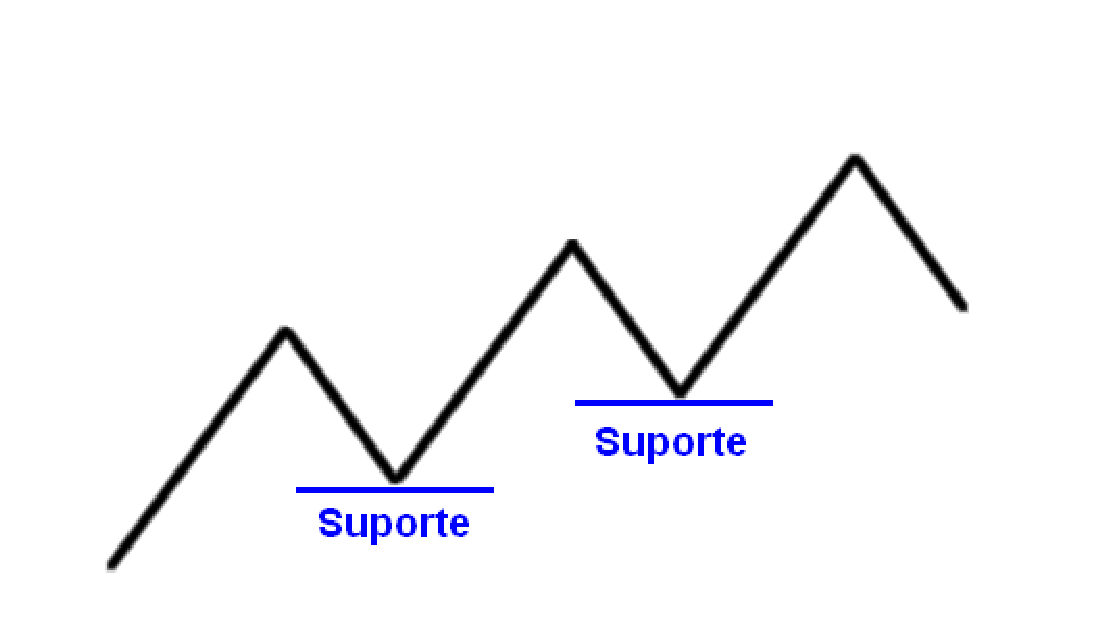
\includegraphics[width=0.9\textwidth]{figuras/retaSuporte}
\caption{Reta de Suporte.}{Fonte: \citeonline[p.~22]{matsura2006}.}
\label{retaSuporte}
\end{figure}

Suporte é uma região gráfica que após uma queda, os preços param e revertem no sentido contrário. É uma área em que os investidores tendem a comprar \cite[p~97]{debastini2008}.

Os níveis de Suporte indicam as cotações em que os investidores acreditam que vão subir. À medida em que as cotações se deslocam para a zona de Suporte, os investidores estão mais confiantes para comprar \cite{collins2012}.

\subsection{Resistência}

Resistência é a região do gráfico em que após um movimento de alta, os preços param e revertem no sentido contrário. É um ponto em que os investidores tende a vender para ter o maior lucro possível \cite[p.~98]{debastini2008}.

Segundo \citeonline[p.~23]{matsura2006}, Resistência representa o nível de preço no qual a pressão vendedora supera a compradora e interrompe o movimento de alta. A Resistência é identificada por uma linha reta horizontal, conforme a figura \ref{retaResistencia}.

\begin{figure}[H]
\centering
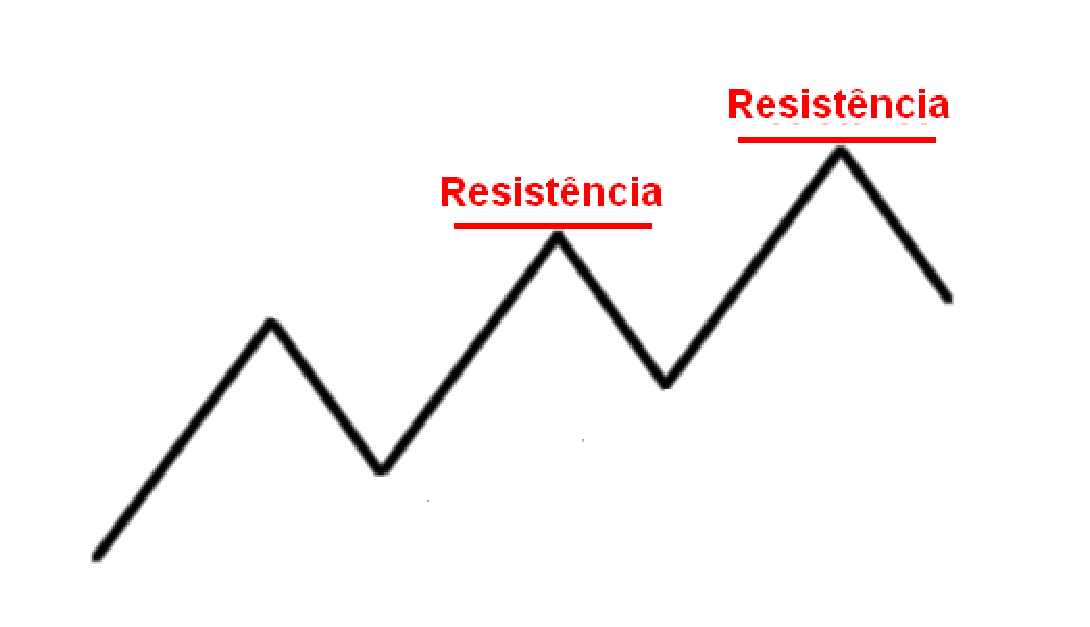
\includegraphics[width=0.5\textwidth]{figuras/retaResistencia}
\caption{Reta de Resistência.}{Fonte: \citeonline[p.~23]{matsura2006}} 
\label{retaResistencia}
\end{figure}

A Resistência indica os níveis das cotações em que os investidores acreditam que as mesmas vão descer. À medida que as cotações se deslocam para a zona de Resistência, os investidores estão mais confiantes para vender \cite{collins2012}.

\section{Métodos Matemáticos}

Métodos Matemáticos é qualquer método que se utiliza da matemática para resolver um problema. É possível citar alguns exemplos desses métodos como equações polinomiais, identidades trigonométricas, geometria coordenada, frações parciais, expansões binomiais, entre outros \cite{riley2011}.

Métodos Matemáticos são aplicados a área de finanças. Cálculo e álgebra linear são fundamentais para o estudo de matemática financeira e ajuda a compreender a dinâmica de mercado \cite{konis2014}.

Este capítulo irá abordar sobre os Métodos Matemáticos de Mínimos Quadrados, Fibonacci e Correlação Linear de Pearson.

\subsection{Método de Mínimos Quadrados}

O método de Mínimos Quadrados determina o valor mais provável de quantidades não conhecidas em que a soma dos quadrados das diferenças entre valores observados e computados é mínimo \cite[p.~72]{inacio2010}.

Usa-se o método de Mínimos Quadrados para determinar a melhor linha de ajuste que passa mais perto de todos os dados coletados, no intuito de obter a melhor linha de ajuste, de forma que minimize as distâncias entre cada ponto de consumo \cite[p.~46]{dias1985}.

A aplicação do método de Mínimos Quadrados visa deduzir a melhor estimativa de mensurações de n medições idênticas (em condições de “repetitividade”) e não idênticas (em condições de “reprodutividade”). Dessa forma o peso estatístico de um resultado é definido \cite[p.~149]{vuolo1996}.

O desvio vertical do ponto:
\begin{equation}
(x_{i}, y_{i})
\end{equation}
da reta:
\begin{equation}
Y = B0 = B1*X_{i}
\end{equation}
é a altura do ponto menos altura da reta. A soma dos desvios quadrados verticais dos pontos:
\begin{equation}
(x_{1}, y_{1})...(x_{i}, y_{i})
\end{equation}
à reta é portanto:
\begin{equation}
f(B0,B1) = \sum{y_{i} - (B0 + B1 * X_{i})}^2
\end{equation}
\begin{equation}
0 <= i > \infty
\end{equation}

As estimativas pontuais de C0 e C1, representadas por K0 e K1 e denominadas estimativa de Mínimos Quadrados, são aquelas que minimizam f(B0, B1). Em suma,  para qualquer B0 e B1, K0 e K1 são tais que:
\begin{equation}
f(K0,K1) <= f(B0,B1)
\end{equation}

A reta de Regressão Estimativa ou de Mínimos Quadrados é, por conseguinte, a reta cuja equação é :
\begin{equation}
Y = K0 + K1X 
\end{equation}
Como mostrado na figura \ref{equacaoMinimos}\cite[p.~441]{devore2006}.

\graphicspath{{figuras/}}
\begin{figure}[H]
\centering
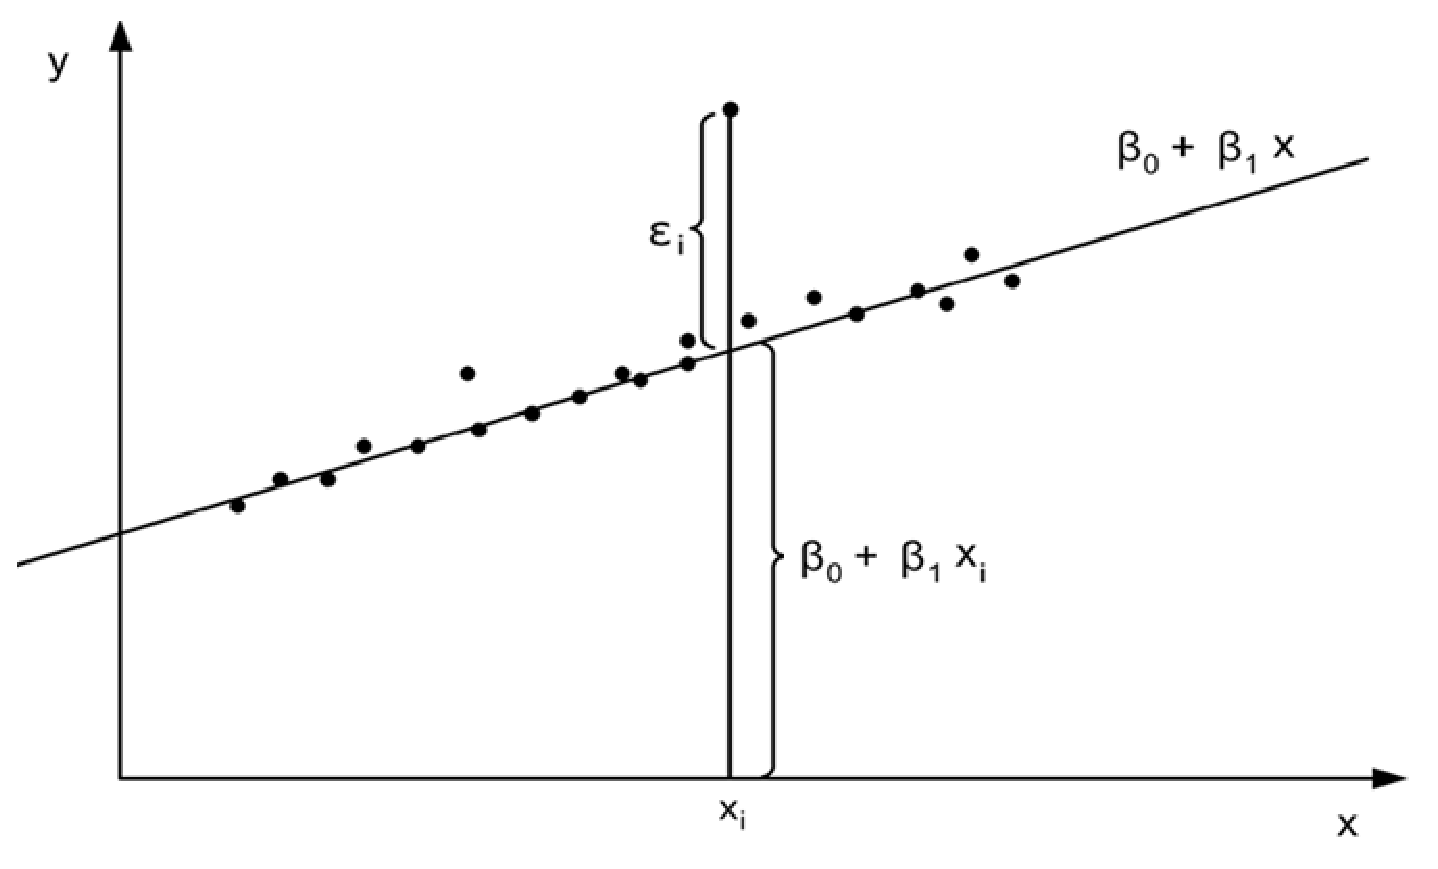
\includegraphics[width=0.5\textwidth]{equacaoMinimosQuadrados}
\caption{Equação da reta Mínimos Quadrados.}{Fonte: \citeonline[p.~443]{devore2006}} 
\label{equacaoMinimos}
\end{figure}

\subsection{Método de Correlação Linear}

Em estudos que envolvem duas ou mais variáveis, é comum o interesse em conhecer o relacionamento entre elas, além das estatísticas descritivas normalmente calculadas. A medida que mostra o grau de relacionamento entre as variáveis é chamada de Coeficiente de Correlação ou Correlação Linear ou Correlação Linear de Pearson. A Correlação Linear também é conhecida como medida de associação, interdependência, intercorrelação ou relação entre as variáveis \cite[p.~62]{lira2004}.

O Coeficiente de Correlação Linear de Pearson (r) é uma estatística utilizada para medir força, intensidade ou grau de relação linear entre duas variáveis aleatórias \cite[p.~664]{ferreira2009}.

Segundo \cite[p.~134]{lopes2005}, a Correlação Linear indica a relação entre duas variáveis. De modo a interpretar o coeficiente de correlação (r), podem ser utilizados os seguintes critérios para classificar os resultados obtidos:

\begin{itemize}
\item De 0 a 0,50: fraca correlação; 
\item De 0,51 a 0,84: moderada correlação;
\item A partir de 0,85: forte correlação.
\end{itemize}

\graphicspath{{figuras/}}
\begin{figure}[H]
\centering
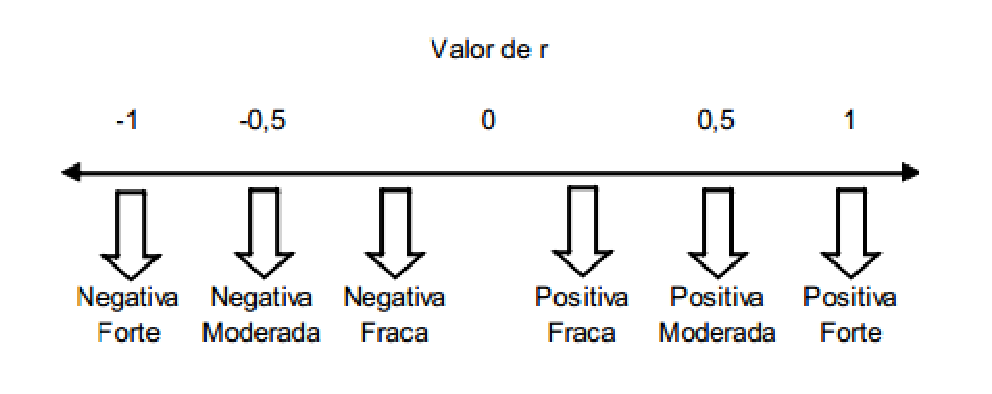
\includegraphics[width=0.5\textwidth]{classificacaoCorrelacaoLinear}
\caption{Classificação da Correlação Linear.}{Fonte: \citeonline[p.~134]{lopes2005}} 
\label{classificacaoCorrelacaoLinear}
\end{figure}

Segundo \citeonline[p.~47]{regra2010} a Correlação Linear revela o grau de associação entre duas variáveis aleatórias. A dependência de duas variáveis X e Y é dada pelo Coeficiente de Correlação Amostral, conhecido também por coeficiente r-de-Pearson. Designa-se, normalmente, por r e é determinado de acordo com a figura \ref{determinacaoCorrelacao}

\graphicspath{{figuras/}}
\begin{figure}[H]
\centering
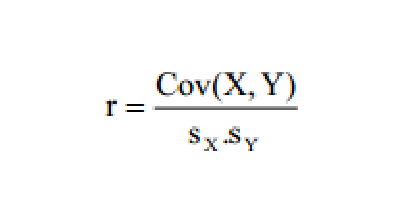
\includegraphics[width=0.5\textwidth]{determinacaoCorrelacao1}
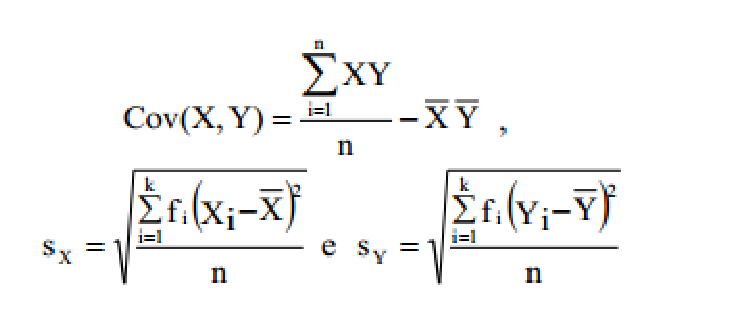
\includegraphics[width=0.5\textwidth]{determinacaoCorrelacao2}
\caption{Determinação da Correlação Linear.}{Fonte:  \citeonline{regra2010}} 
\label{determinacaoCorrelacao}
\end{figure}

Segundo \citeonline[p.~8]{viale2009} as propriedades mais importantes do Coeficiente de Correlação são:

\begin{enumerate}
\item O intervalo de variação vai de -1 a +1.
\item O coeficiente é uma medida adimensional, isto é, independente das unidades de medida das variáveis X e Y.
\item  Quanto mais próximo de +1 for “r”, maior o grau de relacionamento linear positivo entre X e Y, ou seja, se X varia em uma direção, Y variará no mesmo sentido.
\item Quanto mais próximo de -1 for “r”, maior o grau de relacionamento linear negativo entre X e Y, isto é, se X varia em um sentido, Y variará na direção inversa.
\item Quanto mais próximo de zero estiver “r”, menor será o relacionamento linear entre X e Y. Um valor igual a zero indicará ausência apenas de relacionamento linear.
\end{enumerate}


A análise da Correlação Linear fornece um número, indicando como duas variáveis variam conjuntamente e mede a intensidade e a direção da relação linear ou não-linear entre duas variáveis. Essa análise também é um indicador que atende à necessidade de estabelecer a existência ou não de uma relação entre essas variáveis sem que, para isso, seja preciso o ajuste de uma função matemática. Em suma, o grau de variação conjunta entre X e Y é igual ao de Y e X \cite[p.~65]{lira2004}.

\subsection{Método de Fibonacci}

A sucessão ou sequência de Fibonacci é uma sequência de números naturais, na qual os primeiros dois termos são 0 e 1, e cada termo subsequente corresponde à soma dos dois precedentes. A sequência tem o nome do matemático pisano do século XIII Leonardo de Pisa,  conhecido como Leonardo Fibonacci, e os termos são chamados números de Fibonacci. Os números de Fibonacci compõem a seguinte sequência de números inteiros: 0, 1, 1, 2, 3, 5, 8, 13, 21, 34, 55, 89, 144, …, \cite[p.~6]{gagliardi2013}.

Devido a sequência de Fibonacci ser recursiva, é possível determinar uma fórmula capaz de encontrar o valor de qualquer número de Fibonacci, Fn, se seu lugar na sequência, n, for conhecido. Esta propriedade garante que para obter todas as soluções da equação recursiva de Fibonacci: Fn+1 = Fn-1 + Fn, para qualquer n > 1 \cite[p.~12]{sousa2012}.

Segundo \citeonline[p.~32]{rocha2008}, a fórmula de Fibonacci, sem uso da recorrência, é dada de acordo com a figura 5. Essa fórmula também é conhecida como fórmula de Binet.
